\section{Workflow di sviluppo}
TensorFlow Lite, insieme a TensorFlow, offre tutti gli strumenti per la generazione e l’utilizzo di un modello di Machine Learning. Il workflow di
sviluppo è il seguente:
\begin{itemize}
    \item Generazione di un modello TensorFlow Lite: a questo scopo, si può decidere se utilizzare un modello di TensorFlow Lite esistente, creare un
    modello TensorFlow Lite da zero o convertire un modello TensorFlow in un modello TensorFlow Lite. In questo report, si analizzerà l’ultima delle 3
    opzioni poiché coerente con il progetto;
    \item Inferenza: il processo di esecuzione di un modello TensorFlow Lite sul dispositivo per effettuare previsioni basate sui dati di input prende
    nome di inferenza;
    \item Analisi e miglioramento delle prestazioni: tramite dei delegati, si utilizza l’accelerazione hardware in modo che il modello incontri requisiti
    di efficienza elevati.
\end{itemize}

\subsection{Generazione di un modello TensorFlow Lite}
TensorFlow Lite rappresenta i modelli in uno speciale formato portatile efficiente noto come \textbf{FlatBuffers} (identificato dall'estensione del file .tflite ).
Questa scelta offre numerosi vantaggi rispetto al formato del modello di buffer del protocollo di TensorFlow come: dimensioni ridotte
(codice meno ingombrante) e inferenza più rapida (accesso diretto ai dati senza un ulteriore passaggio di analisi/decompressione) che consente a TensorFlow
Lite di funzionare in modo efficiente su dispositivi mobili, che hanno disponibilità di calcolo e memoria limitate.

Un modello TensorFlow Lite, inoltre, può contenere i cosiddetti “metadati” che forniscono una descrizione del modello leggibile dall’uomo e dei dati
interpretabili dalla macchina per la creazione automatica di pipeline di pre e post-elaborazione durante l’inferenza sul dispositivo.
Come è stato anticipato, i principali metodi di generazione di un modello TensorFlow Lite sono 3: 
\begin{enumerate}
    \item Riciclare un modello pre-esistente TensorFlow Lite con o senza metadati;
    \item Creare un modello TensorFlow Lite da zero tramite l’ausilio della libreria TensorFlow Lite Model Maker che semplifica il processo di training di
    un modello TensorFlow Lite utilizzando un set di dati personalizzato;
    \item Conversione di modello TensorFlow in un modello TensorFlow Lite utilizzando il convertitore TensorFlow Lite.
\end{enumerate}

Ci si concentrerà su quest’ultima opzione, in quanto è interessante studiare i meccanismi con cui viene trasformato un modello TensorFlow
(adatto per dispositivi di vario genere e potenza) in un modello TensorFlow Lite (usato per dispositivi mobili e, quindi, molto più limitati in termini
di memoria e risorse di calcolo).

La \textbf{conversione dei modelli} TensorFlow nel formato TensorFlow Lite prevede percorsi diversi a seconda del contenuto del modello di Machine Learning.
Come primo passaggio di tale processo, infatti, è necessario valutare il modello per determinare se può essere convertito direttamente.
Questa valutazione determina se il contenuto del modello è supportato dagli ambienti di runtime TensorFlow Lite standard in base alle operazioni
TensorFlow che utilizza. Se il modello utilizza operazioni non presenti nel set supportato, vi è la possibilità di eseguire il refactoring del modello
o utilizzare delle tecniche di conversione avanzate.

La \textbf{valutazione della conversione} è un passaggio importante prima di provare a convertire il modello. Durante la valutazione, infatti,
si determina se il contenuto del modello è compatibile con il formato TensorFlow Lite in termini di dimensione dei dati utilizzati, requisiti di
elaborazione hardware e dimensioni e complessità del modello. 
La maggior parte dei modelli può essere convertita direttamente nel formato TensorFlow Lite, ma alcuni modelli potrebbero necessitare di un refactoring o
di una conversione avanzata per renderli compatibili.
La conversione vera e propria avviene tramite il \textbf{convertitore TensorFlow Lite} che prende un modello TensorFlow e genera un modello TensorFlow Lite
in formato FlatBuffer. Il convertitore funziona con i seguenti formati del modello di input: SavedModel (modello TensorFlow salvato su disco come un
insieme di file), modello Keras (creato utilizzando l'API di alto livello Keras), formato Keras H5 (una variante del SavedModel supportato dall’API Keras)
e modelli creati tramite delle funzioni concrete (ossia tramite API TensorFlow di basso livello).

\begin{figure}[ht]
    \centering
    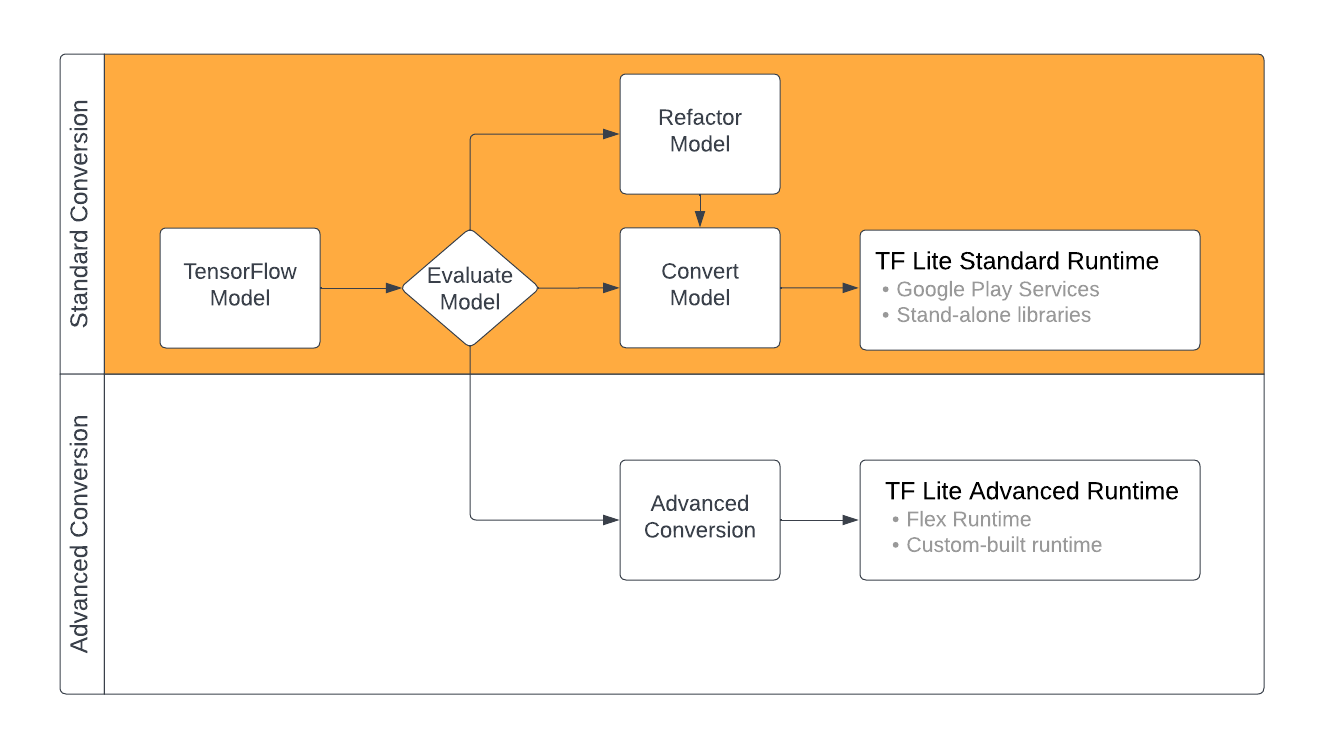
\includegraphics[width=0.8\textwidth]{Immagini/workflow.png}
    \caption{Workflow di conversione di TensorFlow Lite}
    \label{fig:workflow}
\end{figure}

Il modello può essere convertito utilizzando l’\textbf{API Python} o anche lo strumento della riga di comando. E’ consigliato l’utilizzo dell’API Python perché
consente di integrare la conversione nella pipeline di sviluppo, applicare ottimizzazioni, aggiungere metadati e altre ulteriori attività che
semplificano il processo di conversione. La riga di comando, invece, supporta solo la conversione del modello di base.
L’API Python usa, in particolare, la classe \textbf{TF.lite.TFLiteConverter} e i sui metodi \texttt{from\_saved\_model()}, \texttt{from\_keras\_model()} e \texttt{from\_concrete\_functions()}
per convertire modelli rispettivamente di tipo SavedModel, Keras e da funzioni concrete.

Il convertitore accetta, inoltre, 3 opzioni (o flag) che personalizzano la conversione del modello:
\begin{itemize}
    \item I flag di compatibilità che specificano se la conversione deve consentire operatori personalizzati, nel caso in cui nel modello
    TensorFlow vi siano delle operazioni non supportate da TensorFlow Lite;
    \item I flag di ottimizzazione che specificano il tipo di ottimizzazione da applicare durante la conversione. Tendenzialmente la quantizzazione
    è la tecnica maggiormente usata;
    \item I flag di metadati che permettono l’aggiunta di metadati al modello convertito.
\end{itemize}
Nel caso in cui vi siano problemi di compatibilità con gli operatori, si può proporre la \textbf{conversione avanzata}, che prevede il refactoring del
modello e ulteriori opzioni alternative.

\subsection{Ottimizzazione del modello}
Per andare incontro alla limitatezza della memoria e della potenza di dispositivi mobili ed Edge, TensorFlow Lite fornisce delle \textbf{tecniche
di ottimizzazione} per far rientrare i modelli in questi vincoli.
I modi principali in cui l’ottimizzazione del modello aiuta lo sviluppo dell’applicazione sono:
\begin{itemize}
    \item Riduzione delle dimensioni: i modelli più piccoli dispongono di dimensioni di archiviazione ridotte sul dispositivo mobile dell’utente,
    dimensioni di download inferiori in termini di tempo e larghezza di banda e meno utilizzo della memoria RAM durante l’esecuzione, garantendo
    prestazioni e stabilità migliori.
    \item Riduzione della latenza: la diminuzione della quantità di tempo necessaria per eseguire una singola inferenza con un determinato modello
    (latenza) è sintomo di buone prestazioni. La latenza, inoltre, può avere impatto sul consumo energetico ed è importante, dunque, tenere questa
    caratteristica in considerazione;
    \item Compatibilità con l’acceleratore: l’ottimizzazione di un modello permette, in alcuni casi, di utilizzare acceleratori hardware estremamente
    efficienti e veloci.
\end{itemize}
L’ottimizzazione può, però, comportare modifiche nell’accuratezza del modello, che devono essere tenute in considerazione durante il processo di sviluppo di
un’applicazione. Queste variazioni di precisione dipendono molto dall’ottimizzazione del singolo modello e, per questo, non sono facili da prevedere.
In genere, però, i modelli ottimizzati su dimensioni o latenza perdono sempre una quantità variabile di precisione (tendenzialmente piccola). 
Ci sono diversi tipi di ottimizzazione, ma quelli più usati sono:
\begin{itemize}
    \item Quantizzazione: tecnica di ottimizzazione che funziona riducendo la precisione dei valori usati per rappresentare i parametri di un modello,
    che di default sono numeri in virgola mobile a 32 bit. In base ai requisiti dei dati, la richiesta di dimensione, la precisione e l’hardware supportato vi
    sono 4 tipi di quantizzazione: float16 post-training, gamma dinamica post-training, intera post-training e training consapevole della quantizzazione.
    Ogni tipologia è specifica per determinate casistiche ma, in generale, tutti e 4 i tipi di quantizzazione portano ad una riduzione della latenza e delle
    dimensioni a discapito della precisione del modello;
    \item Pruning: metodologia di ottimizzazione che funziona rimuovendo i parametri all’interno di un modello che hanno solo un impatto minimo sulle
    sue previsioni. In questo modo il modello avrà le stesse dimensioni e la stessa latenza di runtime ma potrà essere compresso in maniera più efficace
    e, quindi, sarà più facile ridurre le dimensioni di download;
    \item Clustering: strategia di ottimizzazione che prevede il raggruppamento dei pesi di ciascun livello di un modello in un numero predefinito di
    cluster e, per ogni gruppo, il calcolo del valore del centroide. In questo modo, si riduce il numero dei pesi e quindi si diminuisce la complessità.
    I modelli a cui è stata applicata questa tecnica possono essere compressi più efficacemente.
\end{itemize}

\subsection{Eseguire l'inferenza}
Una volta ottenuto il modello addestrato è possibile testarlo con operazioni di inferenza, ossia il processo di generazione di stime del modello per nuovi
non usati per la fase di training. Nel caso di TensorFlow Lite l’inferenza può essere eseguita in due modi diversi in base al tipo di modello:
\begin{itemize}
    \item Nel caso di \textbf{modelli senza metadati} si può utilizzare l’API dell’interprete TensorFlow Lite;
    \item Nel caso di \textbf{modelli con metadati} è possibile far ricorso a API predefinite utilizzando le Task Library di TensorFlow Lite o
    costruire delle pipeline di inferenza personalizzate con le librerie di supporto di TensorFlow Lite.
\end{itemize}
Per eseguire un’inferenza in un modello TensorFlow Lite è necessario un \textbf{interprete}, il quale deve essere snello e veloce garantendo minima
latenza di carico, di inizializzazione ed esecuzione. L’inferenza in TensorFlow Lite segue i seguenti passaggi:
\begin{enumerate}
    \item Caricamento del modello che contiene il grafo di esecuzione;
    \item Costruzione di un interprete e trasformazione del formato dei dati di input grezzi in un formato supportato dal modello;
    \item Esecuzione dell’inferenza, utilizzando apposite API per l’allocazione dei tensori;
    \item Interpretare l’output in un modo significativo che sia utile nell’applicazione.
\end{enumerate}
Le API di inferenza di TensorFlow sono supportate da Android, iOS e Linux in più linguaggi di programmazione. L’esecuzione di un’inferenza (ma anche
la costruzione di modelli) può far uso di specifiche librerie che aiutano lo sviluppatore a creare esperienze Machine Learning migliori. 
Queste librerie si suddividono in: \textbf{task libraries} e \textbf{support libraries}.

\subsection{Task libraries di TensorFlow Lite}
Le task libraries di TFLite forniscono interfacce ottimizzate per modelli per attività frequenti di Machine Learning, come classificazione di immagini,
domande e risposte, ecc. Le interfacce sono progettate specificamente per ciascuna attività per ottenere le migliori prestazioni e usabilità. La libreria
attività funziona su più piattaforme ed è supportata su Java, C++ e Swift.
Quali sono le caratteristiche di una task library?
\begin{itemize}
    \item API ben definite utilizzabili anche da non esperti di machine learning: È possibile eseguire l’inferenza in sole 5 righe di codice. Le API
    fornite sono potenti e facili da usare, e permettono il facile sviluppo di modelli di machine learning su dispositivi mobili;
    \item Elaborazione dei dati complessa ma efficace: supporta la logica di elaborazione del linguaggio naturale per la conversione dei dati nel
    formato richiesto dal modello. Questa logica è usabile anche nell’addestramento e nell’inferenza;
    \item Aumento della performance: l’elaborazione dei dati viene eseguita in pochi millisecondi, assicurando inferenze rapide e poco costose;
    \item Estendibilità e personalizzazione: è possibile sfruttare tutte i vantaggi forniti dalle task libraries e creare facilmente API personalizzate
    di inferenza Android/iOS.
\end{itemize}

Grazie a queste efficienti librerie, sono supportate diverse attività tra cui: API di visione (come un classificatore di immagini o un rilevatore di
oggetti), di linguaggio naturale, di audio e personalizzate.

\subsection{Support libraries di TensorFlow Lite}
Gli sviluppatori di applicazioni per dispositivi mobili interagiscono con oggetti tipizzati come bitmap o con primitive come gli interi. TensorFlow Lite,
però, usa tensori nella forma di ByteBuffer che sono difficili da debuggare e manipolare. Le support libraries Android di TensorFlow Lite nascono proprio
da questa necessità di supportare l’elaborazione di input e di output di modelli TFLite, rendendo l’interprete più facile da usare.
Le librerie di supporto TensorFlow Lite forniscono, per esempio, una serie di metodi di manipolazione delle immagini base (ritagli/ridimensionamenti) e
di elaborazione di dati audio di base.
